%%%%%%%%%%%%%%%%%%%%%%%%%%%%%%%%%%%%%%%%%%%
%%%%%%  STYLE 29
%%%%%%%%%%%%%%%%%%%%%%%%%%%%%%%%%%%%%%%%%%%
 \cxset{style29/.style={
 name={},
 numbering=arabic,
 number font-size=\normalsize,
 number font-family=\sffamily,
 number font-weight=\bfseries,
 number before={\vspace*{50pt}},
 number position=leftname,
 number after=\vskip-7.5pt,
 chapter font-family=\sffamily,
 chapter font-weight=,
 chapter font-size=\small,
 chapter before={\vskip2.5pt},
 chapter after={\thinrule\par},
 chapter color={black!90},
 number color=\color{black!90},
 title beforeskip={},
 title afterskip={\bigskip},
 title before=,
 title after={\par},
 title font-family=\rmfamily,
 title font-color=\color{black!80},
 title font-weight=\bfseries,
 title font-size=\huge},
 section indent=0pt,
 section font-family=\rmfamily,
 section font-shape=\upshape}
\cxset{style29}

\chapter{Introduction to Style Twenty Nine}
\bigskip\bigskip

\textit{Lambert Schoemacher}
\bigskip\bigskip\bigskip\bigskip

\section{Introduction}
The interesting part of this style is that it uses roman numerals to display the counter that is in a different font than that used for the chapter name.
\medskip

\begin{figure}[ht]
\centering
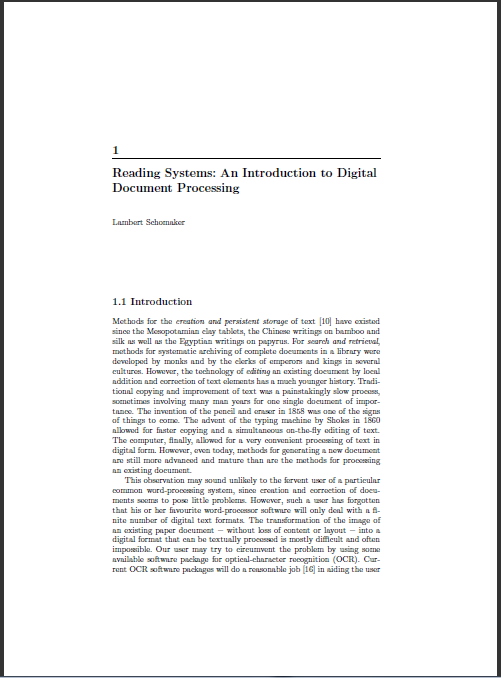
\includegraphics[width=0.6\textwidth]{./chapters/chapter29}
\end{figure}
\lipsum[3]

